\subsubsection{XML Import}
\paragraph{Reason For Component}

The general idea with this utility is to import XML files into the a configured database. This will take any XML file or input stream convert them into Java objects and then store them into an SQL database. The interface to this utility is an intuitive user interface where you can open, preview and import files. The interface had to be intuitive enough for a non-computer science audience. 


\paragraph{Design}
\begin{figure}[h]
	\centering
		\includegraphics[width=3.00in]{Images/ImportUse.jpg}
	\caption{The Use Case For The Import Utility}
	\label{fig:Import Use}
\end{figure}
\par
The first design choice we made was to use Java Swing components to develop our user interface, so we could use the standard components in the Swing library. These components have been well tested and are familiar to the user. The second design choice was to use pre-configured JaxB and Hibernate properties. The import utility assumes that hibernate has been properly configured and the JaxB classes exist. The hibernate and JaxB configurations are required upon loading. Error messages received by the utility are likely to be because the database or hibernate properties have not been configured correctly, or the utility cannot find the JaxB classes. 
\par
The XML Import utility is made up of two classes: the ImportPanel for the user interface, and the ImportEngine for the logic. We chose this design to have interface separated from functionality. We wanted the ImportEngine to be removable from the GUI so developers can take that class and use it with other user interfaces. 
\par
The user interface includes: a text area for previewing XML files, an open dialog for opening XML files, a text area to view an opened file path, an open button, an import button, and a preview button. Files can be opened via a file dialog by clicking open button. The open dialog that has a default filter for XML files for ease of use. Once opened, the file can be previewed by pressing the preview button or imported using the import button. When a preview is performed on a large file, a progress monitor pops up to give the user feedback on how long the action will take. 
\begin{figure}[h]
	\centering
		\includegraphics[width=1.00\textwidth]{Images/ImportScreenshot2.jpg}
	\caption{A screen shot of the import interface}
	\label{fig:ImportScreenshot}
\end{figure}


\par	
When the import button is pressed a new ImportEngine is created. The ImportEngine takes a hibernate configuration and a JaxB context path. The loadToDB method called which converts the xml to Java objects then uses hibernate to commit the data to the SQL database. A detailed class diagram is shown below. A progress monitor opens, however, it did not perform as specified in Swing. This will be addressed in the next version

\begin{figure}[h]
	\centering
		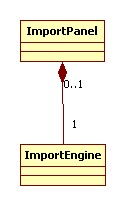
\includegraphics[width=4.00in]{Images/ImportClasses.jpg}
	\caption{The ImportEngine is part of the ImportPanel but it can also run stand-alone}
	\label{fig:ImportClasses}
\end{figure}

\paragraph{Evaluation}
The module and design worked well from the start. Most of our problems were with our build tool, ANT, and making small changes to the user interface. We went through several iterations with the panel to make it more usable and to fix bugs. We had to learn the how to save objects to the database using hibernate as the middle ware to create the ImportEngine. Hibernate performed very well, and the ImportEngine required only minor changes after the first coding iterations. We was a little disappointed with the Java components that we tried to use for user feedback, specifically the progress monitor for input streams. Though it worked well for previewing large XML files, it did not work as expected for giving feedback during a large import. Overall, the utility performed well. 

\paragraph{What's Next}
We plan to focus on the usability of the interface. We would like to implement a better and consistent user feedback system. There are also performance issues we would like to solve, such as allowing multiple imports to be conducted at the same time and a more seamless configuration with multiple databases. Lastly, we would like to implement tool tips and have a help menu item. 

